\documentclass[12pt]{article}
\usepackage[spanish,mexico]{babel}
	\selectlanguage{spanish}
\usepackage{graphicx}
\usepackage{amsmath}
\usepackage{wrapfig}
\usepackage{float}
\usepackage[utf8]{inputenc}

\usepackage{graphicx}
\graphicspath{{images/}}

%\usepackage{vmargin}
%\setmarginsrb{3 cm}{2.5 cm}{3 cm}{2.5 cm}{1 cm}{1.5 cm}{1 cm}{1.5 cm}

\title{Actividad 4: Ajuste de datos; mínimos cuadrados}
\author{Martín Alejandro Paredes Sosa}
\date{Febrero 2016}


\begin{document}

\maketitle

\section{Introducción}
En el área de la estadística, hay un campo denominado análisis de regresión cuya misión es poder obtener modelos matemáticos, como las funciones, para diversos comportamientos de fenómenos observados. Tras tener una colección de datos, estos se analizan y con diferentes métodos, se llega a facilitar el estudio del fenómeno con funciones conocidas, como las rectas, parábolas o exponenciales.\\

Mínimos cuadrados es una técnica de análisis numérico enmarcada dentro de la optimización matemática, en la que, dados un conjunto de pares ordenados: variable independiente, variable dependiente, y una familia de funciones, se intenta encontrar la función continua, dentro de dicha familia, que mejor se aproxime a los datos (un ``mejor ajuste''), de acuerdo con el criterio de mínimo error cuadrático \cite{Mc}. 

\begin{figure}[H]
\centering
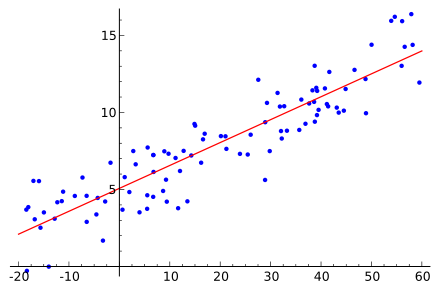
\includegraphics[width=6cm]{AjusteMC.png}
\caption{Ejemplo de una regresión lineal.\cite{a}.}
\end{figure}

La técnica de los mínimos cuadrados es parte de ambas secciones en el análisis de la regresión, pues se puede utilizar tanto en la regresión lineal como en el no lineal. En la actividad de hoy, se utilizaron ambos métodos para poder ajustar funciones del tipo lineal y exponencial a dos conjuntos de datos distintos con una herramienta que nos proporciona el paquete Scipy de Python.\\

El método \textit{scipy.optimze.leastsq} encuentra el conjunto de parámetros que minimizan la función de error. Este comienza a partir de una primera conjetura y trata de minimizar la función de error cada que entran los datos proporcionados, y así devuelve la lista de los parámetros que mejor se ajusten a los datos \cite{Q}. 

\section{Actividad}
En esta practica se realizara un ajuste lineal de temperaturas medias de invierno en Nueva York\cite{Da1} y un ajuste exponencial de la presión atmosférica con respecto a la altura\cite{Da2}, utilizando los paquetes de \textit{Scipy}: \textit{curve\_fit; leastsq}.\\

\subsection{Programa 1: AjLineal.py}
En este programa se lee el documento con los datos de temperaturas medias de invierno en Nueva York\cite{Da1}, y se realiza un ajuste lineal.

\subparagraph{Código: AjLineal.py}
\begin{verbatim}
#importando librerias
import matplotlib.pyplot as plt
import numpy as np
from scipy.optimize import  leastsq

#Obtencion de datos
datos = np.loadtxt('TNY.txt')

#Separacion de los datos para un mejor manejo
x1 = datos[:,0]
y1 = datos[:,1] 

#Ajuste Lineal   

fitfunc = lambda p, x: p[0] + p[1]*x # Target function
errfunc = lambda p, x, y: fitfunc(p, x) - y # Distance to the target function
p0 = [-15., -1.] # Initial guess for the parameters
p1, success = leastsq(errfunc, p0[:], args=(x1, y1))

#Genero datos y grafico
time = np.linspace(x1.min(), x1.max(), 100)
plt.plot(x1, y1, "go", time, fitfunc(p1, time), "b-") # Plot of the data and the fit

#Propiedades de la Grafica
plt.title("Temperatura Nueva York en invierno")
plt.xlabel("Ano")
plt.ylabel("Temperatura")

plt.show()
\end{verbatim}
Lo que resulta de este código es lo siguiente:
\begin{figure}[H]
	\centering
	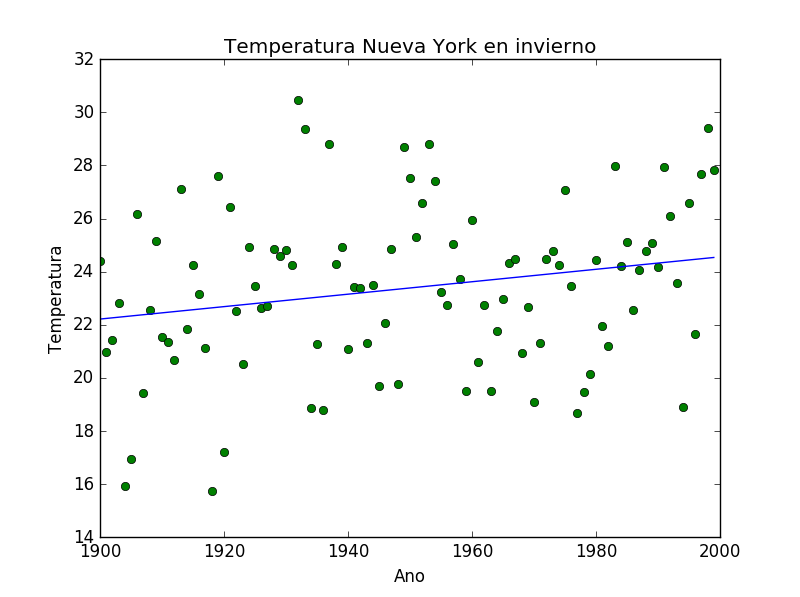
\includegraphics[width=8cm]{AjusteL.png}
	\caption{Ajuste Lineal, Temperatura Nueva York en invierno}
\end{figure}

\subsection{Programa 1: AjExp.py}
En este programa se lee el documento con los datos de la presión atmosférica con respecto a la altura\cite{Da2}, y se realiza un ajuste exponencial.

\subparagraph{Código: AjExp.py}
\begin{verbatim}
#importando librerias
import matplotlib.pyplot as plt
import numpy as np
from scipy.optimize import  curve_fit

#Obtencion de datos
datos = np.loadtxt('PvsA.txt')

#Separacion de los datos para un mejor manejo
x1 = datos[:,0]
y1 = datos[:,1] 

#Definiendo la forma de la función a ajustar
#y=c*e^(-a*x)+b
def f(x,a,b,c):
    return c * np.exp(-a * x) + b

#Optimizacion de la curva
popt, pcov = curve_fit(f,x1,y1)

#Genero datos y grafico

plt.plot(x1, y1, "go", label='Datos')
plt.plot( x1, f(x1, *popt), "b-", label='Ajuste Exponencial')

#Propiedades de la Grafica
plt.grid()
plt.legend()
plt.title("Atmospheric pressure vs. altitude")
plt.xlabel("Altitude")
plt.ylabel("Pressure")

plt.show()
\end{verbatim}
Lo que resulta de este código es lo siguiente:
\begin{figure}[H]
	\centering
	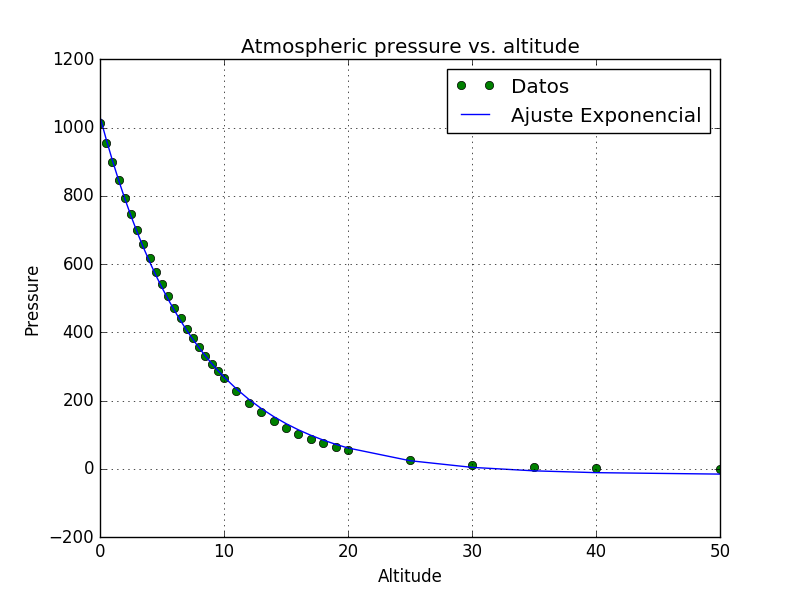
\includegraphics[width=8cm]{AjusteExp.png}
	\caption{Ajuste Exponencial, Presión Atmosférica con Respecto a la Altura}
\end{figure}

\pagebreak

\begin{thebibliography}{9}
	
	\bibitem{Mc}
	Wikipedia,
	\emph{Mínimos cuadrados}. Recuperado de: https://es.wikipedia.org/wiki/M\% C3\% ADnimos\_cuadrados
	
	\bibitem{a}
	Lizárraga, C. (2016)
	\textit{Actividad 4 (2016-1)}. Recuperado de: http://computacional1.pbworks.com/w/page/105016164/Actividad\%204\%20(2016-1)
	

	\bibitem{Q}
	Qiku programación, (2013)
	\emph{Cómo utilizar leastsq función desde scipy.optimize en python}. Recuperado de: http://goo.gl/giZ7rO


	\bibitem{Da1}
	Quantitative Environmental Learning Project, (s.f.)	\emph{New York's Winter Mean Temperature} Recuperado de: http://www.seattlecentral.edu/qelp/sets/048/048.html\# Top
	
	
	\bibitem{Da2}
	Quantitative Environmental Learning Project, (s.f.)	\emph{Earth's Standard Atmosphere}. Recuperado de: http://www.seattlecentral.edu/qelp/sets/024/024.html
	
	\bibitem{RL}
	\emph{Regresión lineal}. (s.f.) Recuperado de: http://www.sc.ehu.es/sbweb/fisica/cursoJava/numerico/regresion/regresion.htm

	\bibitem{RE}
	\emph{Regresión exponencial}.(s.f.) Recuperado de https://www.uv.es/ceaces/base/regresion/exponenci.htm
	
	\bibitem{S1}
	Scipy (2016), 
	\emph{leastsq}. Recuperado de:\\ http://docs.scipy.org/doc/scipy/reference/generated/scipy.optimize.leastsq.html\# scipy.optimize.leastsq

	\bibitem{S2}
	Scipy (2016),
	\emph{curve\_fit}. Recuperado de:\\ http://docs.scipy.org/doc/scipy/reference/generated/scipy.optimize.curve\_fit.html
\end{thebibliography}


\end{document}